\chapter{Introduction}
\pagenumbering{arabic}

\section{Background and Motivation}

Large language models (LLMs) have transformed natural language processing, achieving strong performance on tasks ranging from question answering to mathematical problem-solving and code generation. A critical driver of this success has been \emph{chain-of-thought} (CoT) prompting~\citep{wei2022chain}, which instructs the model to produce intermediate reasoning steps before arriving at a final answer. By making the reasoning process explicit, CoT improves accuracy on multi-step problems and provides a degree of interpretability.

Despite its effectiveness, CoT has a fundamental limitation: it generates reasoning as a \emph{single, linear sequence}. Once a step is generated, the model cannot reconsider it---there is no mechanism for backtracking, comparing alternatives, or revisiting earlier decisions. This creates three classes of failure:

\begin{enumerate}
\item \textbf{Error propagation:} An early mistake compounds through subsequent steps, since each step conditions on all prior content.
\item \textbf{Evidence fragmentation:} Problems requiring integration of multiple independent facts are difficult to solve in a single left-to-right narrative.
\item \textbf{Commitment bias:} The model commits to the first plausible-sounding reasoning path even when alternatives would be better.
\end{enumerate}

These failures motivate \emph{search-based reasoning}, where the model explores multiple partial reasoning traces before committing. Methods such as Tree-of-Thoughts~\citep{yao2024tree}, MCTS-based reasoning~\citep{hao2023reasoning}, and A* search over reasoning traces allow the model to maintain a frontier of promising states, expand the most promising ones, and ultimately select the best complete trace.

However, search introduces its own problems. It is computationally expensive (typically 10--24$\times$ the cost of CoT), and on simple problems it can \emph{hurt} by overthinking---introducing unnecessary distinctions, pursuing spurious associations, or wasting budget on near-duplicate explorations. The central question of this thesis is therefore:

\begin{center}
\fbox{\parbox{0.85\textwidth}{\centering\emph{Which structural properties of a reasoning problem predict whether search-based reasoning will help over chain-of-thought?}}}
\end{center}

\section{The CoT vs. Search Trade-off}

Figure~\ref{fig:paradigm_comparison} illustrates the fundamental architectural difference between CoT and A* search. CoT generates one path; A* maintains a priority queue of partial traces and expands them based on a heuristic estimate of remaining difficulty.

\begin{figure}[htbp]
\centering
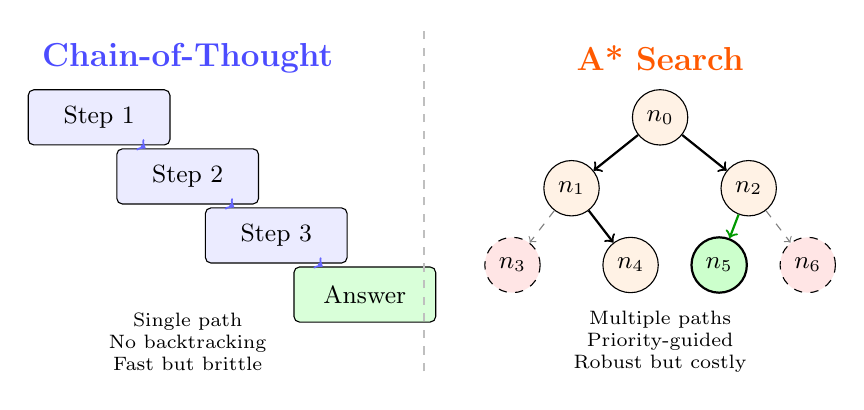
\begin{tikzpicture}[
  scale=0.75,
  every node/.style={font=\small},
  rstep/.style={rectangle, draw, rounded corners=2pt, minimum width=1.8cm, minimum height=0.7cm, fill=blue!8},
  searchnode/.style={circle, draw, minimum size=0.7cm, fill=orange!10},
  goalnode/.style={circle, draw, minimum size=0.7cm, fill=green!20, thick},
  deadnode/.style={circle, draw, minimum size=0.7cm, fill=red!10, dashed},
]

% CoT (left side)
\node[font=\large\bfseries, blue!70] at (-4, 4.5) {Chain-of-Thought};
\node[rstep] (s1) at (-5.5, 3.5) {Step 1};
\node[rstep] (s2) at (-4, 2.5) {Step 2};
\node[rstep] (s3) at (-2.5, 1.5) {Step 3};
\node[rstep, fill=green!15] (s4) at (-1, 0.5) {Answer};
\draw[->, thick, blue!60] (s1) -- (s2);
\draw[->, thick, blue!60] (s2) -- (s3);
\draw[->, thick, blue!60] (s3) -- (s4);
\node[font=\scriptsize, text width=3cm, align=center] at (-4, -0.3) {Single path\\No backtracking\\Fast but brittle};

% A* (right side)
\node[font=\large\bfseries, orange!70!red] at (4, 4.5) {A* Search};
\node[searchnode] (r) at (4, 3.5) {$n_0$};
\node[searchnode] (a) at (2.5, 2.3) {$n_1$};
\node[searchnode] (b) at (5.5, 2.3) {$n_2$};
\node[deadnode] (c) at (1.5, 1) {$n_3$};
\node[searchnode] (d) at (3.5, 1) {$n_4$};
\node[goalnode] (e) at (5, 1) {$n_5$};
\node[deadnode] (f) at (6.5, 1) {$n_6$};
\draw[->, thick] (r) -- (a);
\draw[->, thick] (r) -- (b);
\draw[->, dashed, gray] (a) -- (c);
\draw[->, thick] (a) -- (d);
\draw[->, thick, green!60!black] (b) -- (e);
\draw[->, dashed, gray] (b) -- (f);
\node[font=\scriptsize, text width=3cm, align=center] at (4, -0.3) {Multiple paths\\Priority-guided\\Robust but costly};

% Divider
\draw[thick, dashed, gray!50] (0, -0.8) -- (0, 5);

\end{tikzpicture}
\caption{Comparison of reasoning paradigms. \textbf{Left:} CoT generates a single linear trace---efficient but with no recovery from early errors. \textbf{Right:} A* search maintains a frontier of partial traces (circles), expands the most promising (solid arrows), and prunes dead ends (dashed). Green = goal reached; red dashed = abandoned.}
\label{fig:paradigm_comparison}
\end{figure}

The key insight of this thesis is that \emph{neither paradigm is universally better}. Different problems call for different strategies, and the decision can be made reliably from structural features of the input alone---before generating any reasoning trace.

\section{Motivating Example}

Consider the StrategyQA question: \emph{``Is shrimp scampi definitely free of plastic?''} (gold answer: No).

\begin{figure}[htbp]
\centering
\begin{tcolorbox}[
  enhanced, colback=white, colframe=black!75, boxrule=0.7pt,
  arc=1.8mm, left=6pt, right=6pt, top=6pt, bottom=6pt,
  title=\textbf{Motivating Example}\hfill\emph{``Is shrimp scampi definitely free of plastic?''}\hfill\textbf{Gold: No},
  colbacktitle=black!4, coltitle=black, fonttitle=\small
]
\small

\begin{minipage}[t]{0.47\textwidth}
\textbf{\color{red!75!black} Chain-of-Thought (Incorrect)}\\[4pt]
\textit{Follows a chronological schema, missing the key biological fact.}
\begin{enumerate}[leftmargin=*, itemsep=1pt]
\item Shrimp are caught/farmed; no conclusive evidence of plastic.
\item Processing does not involve contamination.
\item Cooking does not introduce plastic.
\item Regulatory standards make contamination unlikely.
\item \textbf{Answer: Yes} $\times$
\end{enumerate}
\end{minipage}
\hfill
\vrule
\hfill
\begin{minipage}[t]{0.47\textwidth}
\textbf{\color{blue!75!black} A* Search (Correct)}\\[4pt]
\textit{Prioritizes the decisive biological premise directly.}
\begin{enumerate}[leftmargin=*, itemsep=1pt]
\item Shrimp often contain microplastics in tissues.
\item Preparation does not remove pre-existing microplastics.
\item \textbf{Answer: No} $\checkmark$
\end{enumerate}
\vspace{1em}
\textit{Search reached the key fact in fewer, more relevant steps.}
\end{minipage}

\end{tcolorbox}
\caption{CoT pursues a plausible but misdirected chronological analysis, while A* surfaces the decisive evidence (microplastic bioaccumulation) early via heuristic-guided exploration.}
\label{fig:motivating_example_thesis}
\end{figure}

The difference is not that one model ``knew more.'' It is that the search procedure prioritized a more relevant branch of the reasoning space. This pattern repeats systematically: across eight benchmarks, CoT and A* succeed on different instance subsets, and the structural complexity of the problem predicts which will win.

\section{Research Questions}

This thesis addresses four concrete research questions:

\begin{description}[leftmargin=1.5cm, labelwidth=1.2cm]
\item[\textbf{RQ1}] Does guided search (A*) dominate CoT, or do they trade wins across different problem types?
\item[\textbf{RQ2}] When CoT and A* disagree, is the split random or systematic---predictable from problem structure?
\item[\textbf{RQ3}] Can we predict which method will win from structural features of the input alone---before any generation?
\item[\textbf{RQ4}] Does such a pre-generation router outperform post-hoc judges that observe full reasoning traces?
\end{description}

\section{Contributions}

This thesis makes six contributions:

\begin{enumerate}
\item \textbf{Comprehensive multi-domain evaluation.} We compare CoT, A*, Self-Consistency, and Tree-of-Thought across eight benchmarks spanning QA (StrategyQA, LogicQA, HotpotQA), math (GSM8K, MATH), and code generation (HumanEval, MBPP, CodeContests), at three model scales (0.5B, 8B, 14B).

\item \textbf{Quantified complementarity.} We demonstrate that CoT and A* solve genuinely different instance subsets, with oracle gaps of up to 14 percentage points above the best single method.

\item \textbf{Reasoning Topology Framework.} We introduce 13 pre-generation structural features and show that a derived \emph{branching coefficient} predicts A* advantage with $R^2 = 0.94$ on QA/math clusters.

\item \textbf{Topology-aware routing.} A pre-generation router using only structural features recovers 32.3\% of the oracle gap at 8B and 89.7\% on CodeContests at 0.5B---outperforming all trace-based routers.

\item \textbf{Fluency-Correctness Asymmetry.} We identify that in 38\% of disagreement cases, the more fluent trace is wrong, explaining why post-hoc judges are systematically misled.

\item \textbf{Cross-domain transfer.} The topology framework extends to code generation, with multi-return tasks showing a +18.2pp A* advantage at 14B---the code analogue of branching topology.
\end{enumerate}

\section{Scope and Approach}

Our approach is deliberately controlled. We use A* search (not MCTS or beam search) because it cleanly separates the key ingredients of guided search---a priority frontier, a path cost, and a heuristic estimate---without entangling them with evaluator design, rollout policies, or fixed-width pruning. This makes it possible to isolate \emph{when the act of branching itself} is responsible for gains or losses.

Figure~\ref{fig:thesis_overview} provides a high-level overview of the thesis workflow.

\begin{figure}[htbp]
\centering
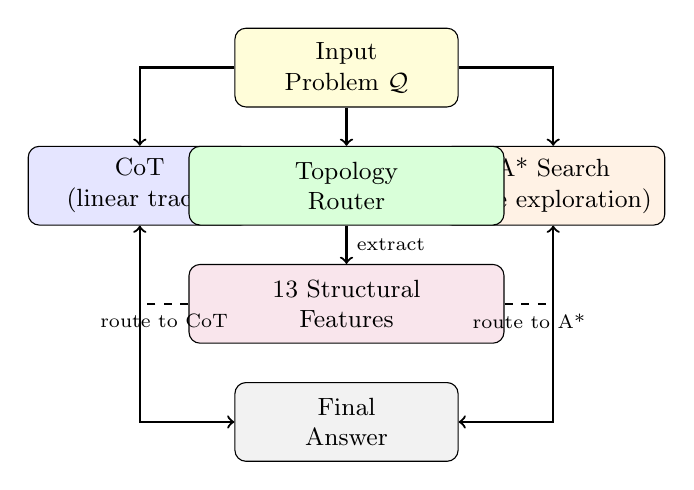
\begin{tikzpicture}[
  scale=0.75,
  every node/.style={font=\small},
  block/.style={rectangle, draw, rounded corners, minimum width=2.8cm, minimum height=1cm, text width=2.6cm, align=center},
]
% Row 1: Input
\node[block, fill=yellow!15] (input) at (0, 0) {Input\\Problem $\mathcal{Q}$};

% Row 2: Two paths
\node[block, fill=blue!10] (cot) at (-3.5, -2) {CoT\\(linear trace)};
\node[block, fill=orange!10] (astar) at (3.5, -2) {A* Search\\(tree exploration)};

% Row 3: Router
\node[block, fill=green!15, minimum width=4cm] (router) at (0, -2) {Topology\\Router};

% Row 4: Features
\node[block, fill=purple!10, minimum width=4cm] (feat) at (0, -4) {13 Structural\\Features};

% Row 5: Output
\node[block, fill=gray!10] (output) at (0, -6) {Final\\Answer};

% Arrows
\draw[->, thick] (input) -- (router);
\draw[->, thick] (input) -| (cot);
\draw[->, thick] (input) -| (astar);
\draw[->, thick] (router) -- (feat) node[midway, right, font=\scriptsize] {extract};
\draw[->, thick, dashed] (feat) -| (cot) node[near start, below, font=\scriptsize] {route to CoT};
\draw[->, thick, dashed] (feat) -| (astar) node[near start, below, font=\scriptsize] {route to A*};
\draw[->, thick] (cot) |- (output);
\draw[->, thick] (astar) |- (output);

\end{tikzpicture}
\caption{Thesis overview. Given an input problem, the topology router extracts 13 structural features and decides whether to use CoT (fast, linear) or A* search (expensive, robust). The routing decision is made \emph{before} any generation.}
\label{fig:thesis_overview}
\end{figure}

\section{Organization of the Thesis}

The remainder of this thesis is organized as follows:

\begin{description}
\item[Chapter 2: Literature Review] covers prior work on chain-of-thought prompting, structured reasoning, search-augmented methods, inference-time compute scaling, and routing strategies.
\item[Chapter 3: Methodology] formalizes the A* search procedure, heuristic design (with admissibility proof), topology feature extraction, and all routing strategies compared in this work.
\item[Chapter 4: Experiments and Results] presents comprehensive results across eight benchmarks and three scales, including topology cluster analysis, router comparison, fluency-correctness asymmetry, and code generation extension.
\item[Chapter 5: Conclusion and Future Work] summarizes findings, discusses limitations, and outlines directions for future research.
\end{description}
